\documentclass[12pt,a4paper]{article}
\usepackage{geometry}
\geometry{left=2.54cm, right=2.54cm, top=2.98cm, bottom=2.98cm}
\usepackage{fancyhdr} 
\usepackage{enumerate}
\usepackage{graphicx}
\usepackage{subfigure}
\usepackage{float}
\usepackage{indentfirst}
\usepackage{threeparttable}
\usepackage{hyperref}
\hypersetup{
    colorlinks=true,
    linkcolor=blue,
    filecolor=magenta,      
    urlcolor=cyan,
    pdfpagemode=FullScreen,
    }
\title{Physics Lab Report}
\author{ZHANGYIHENG 10.7 27}
\begin{document}
\maketitle
\begin{center}
\tableofcontents
\end{center}
\setlength{\parindent}{4ex}


\newpage
\section{Introduction}
\subsection{Purpose}
The objective of the investigation is to figure out is there a valid 
relationship between the velocity and displacement of a free-falling object.\par



\subsection{Laborartory Apparatuses}
\begin{enumerate}
    \item The falling object
    \item Ticker-timer
    \item Paper tape
    \item A stand
    \item A clamp
    \linespread{0.5}
\end{enumerate}

\begin{figure}[H]
    \subfigure[clamp and paper tape]{
    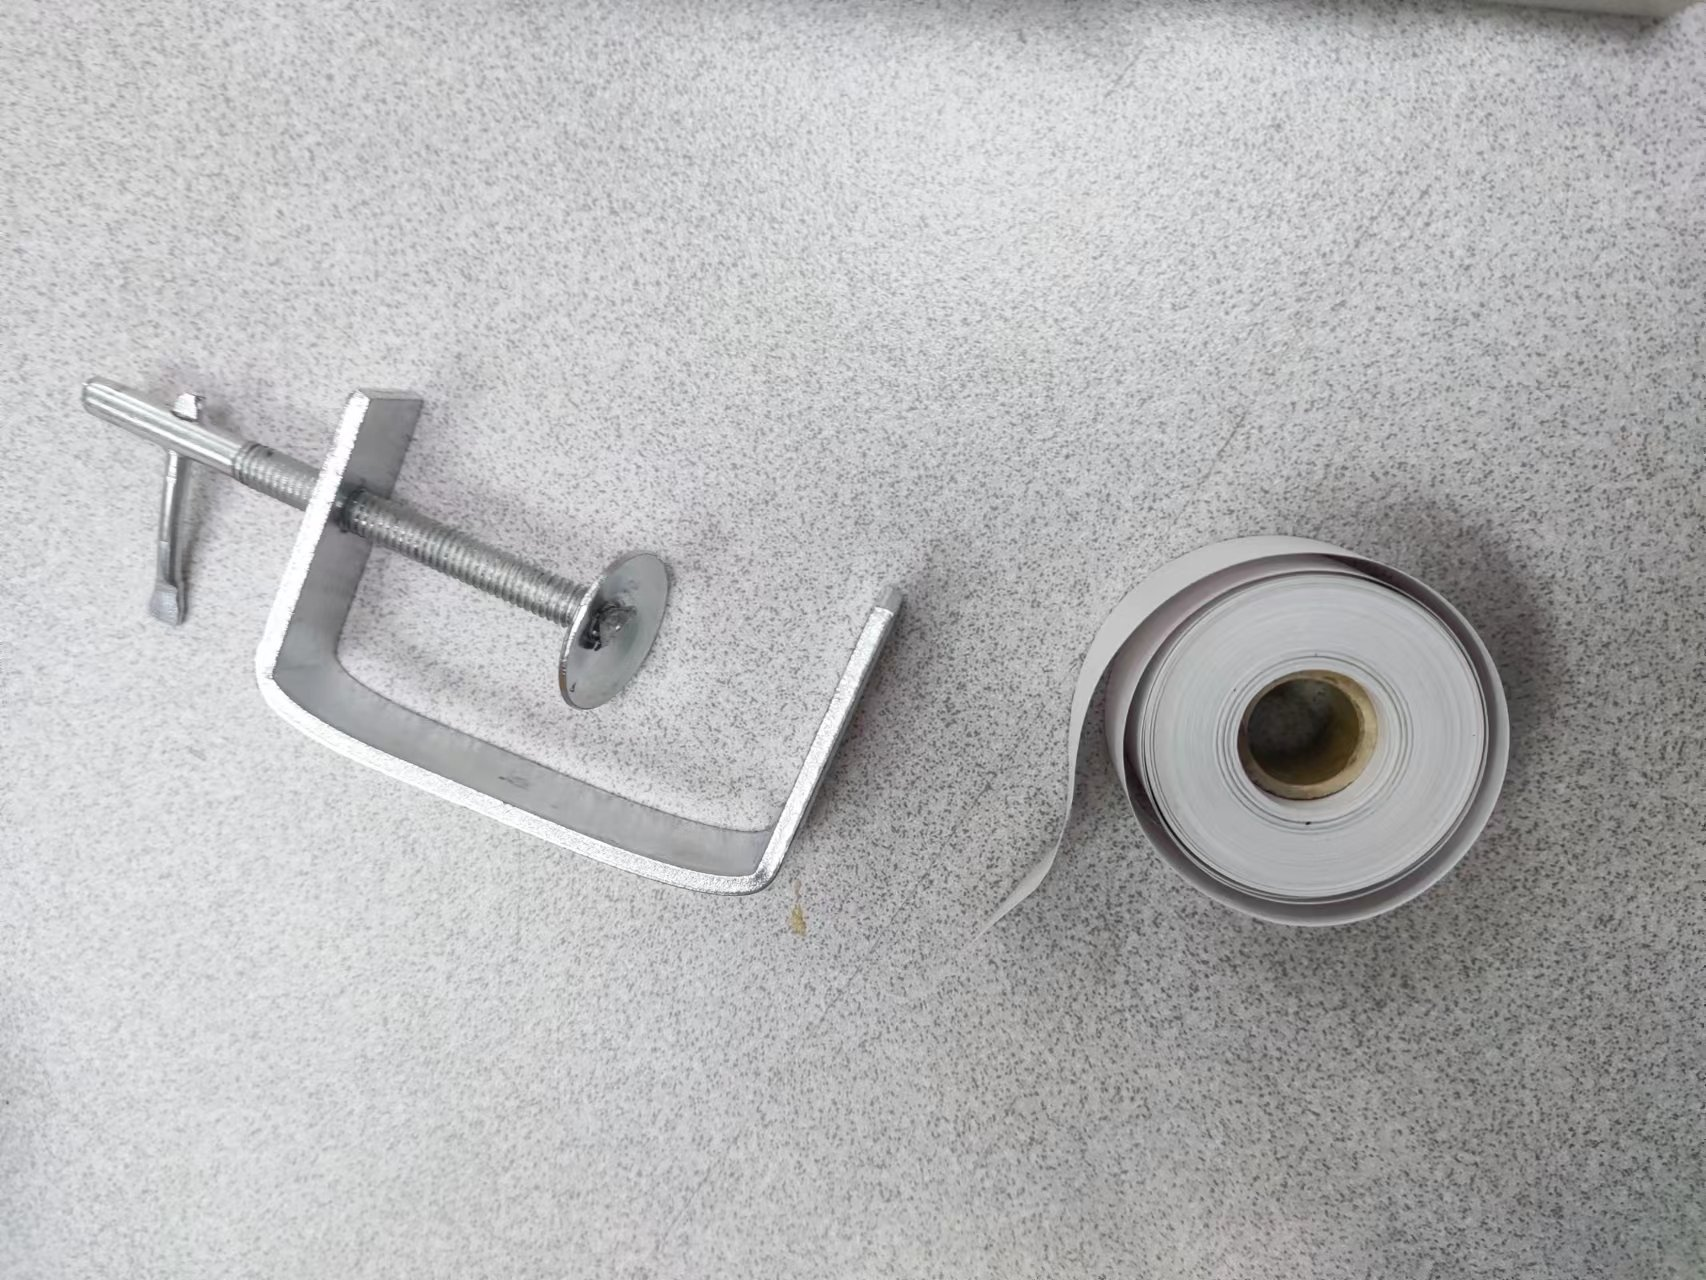
\includegraphics[width=0.35\textwidth]{2601669167979_.pic.jpg}}
    \subfigure[falling object]{
    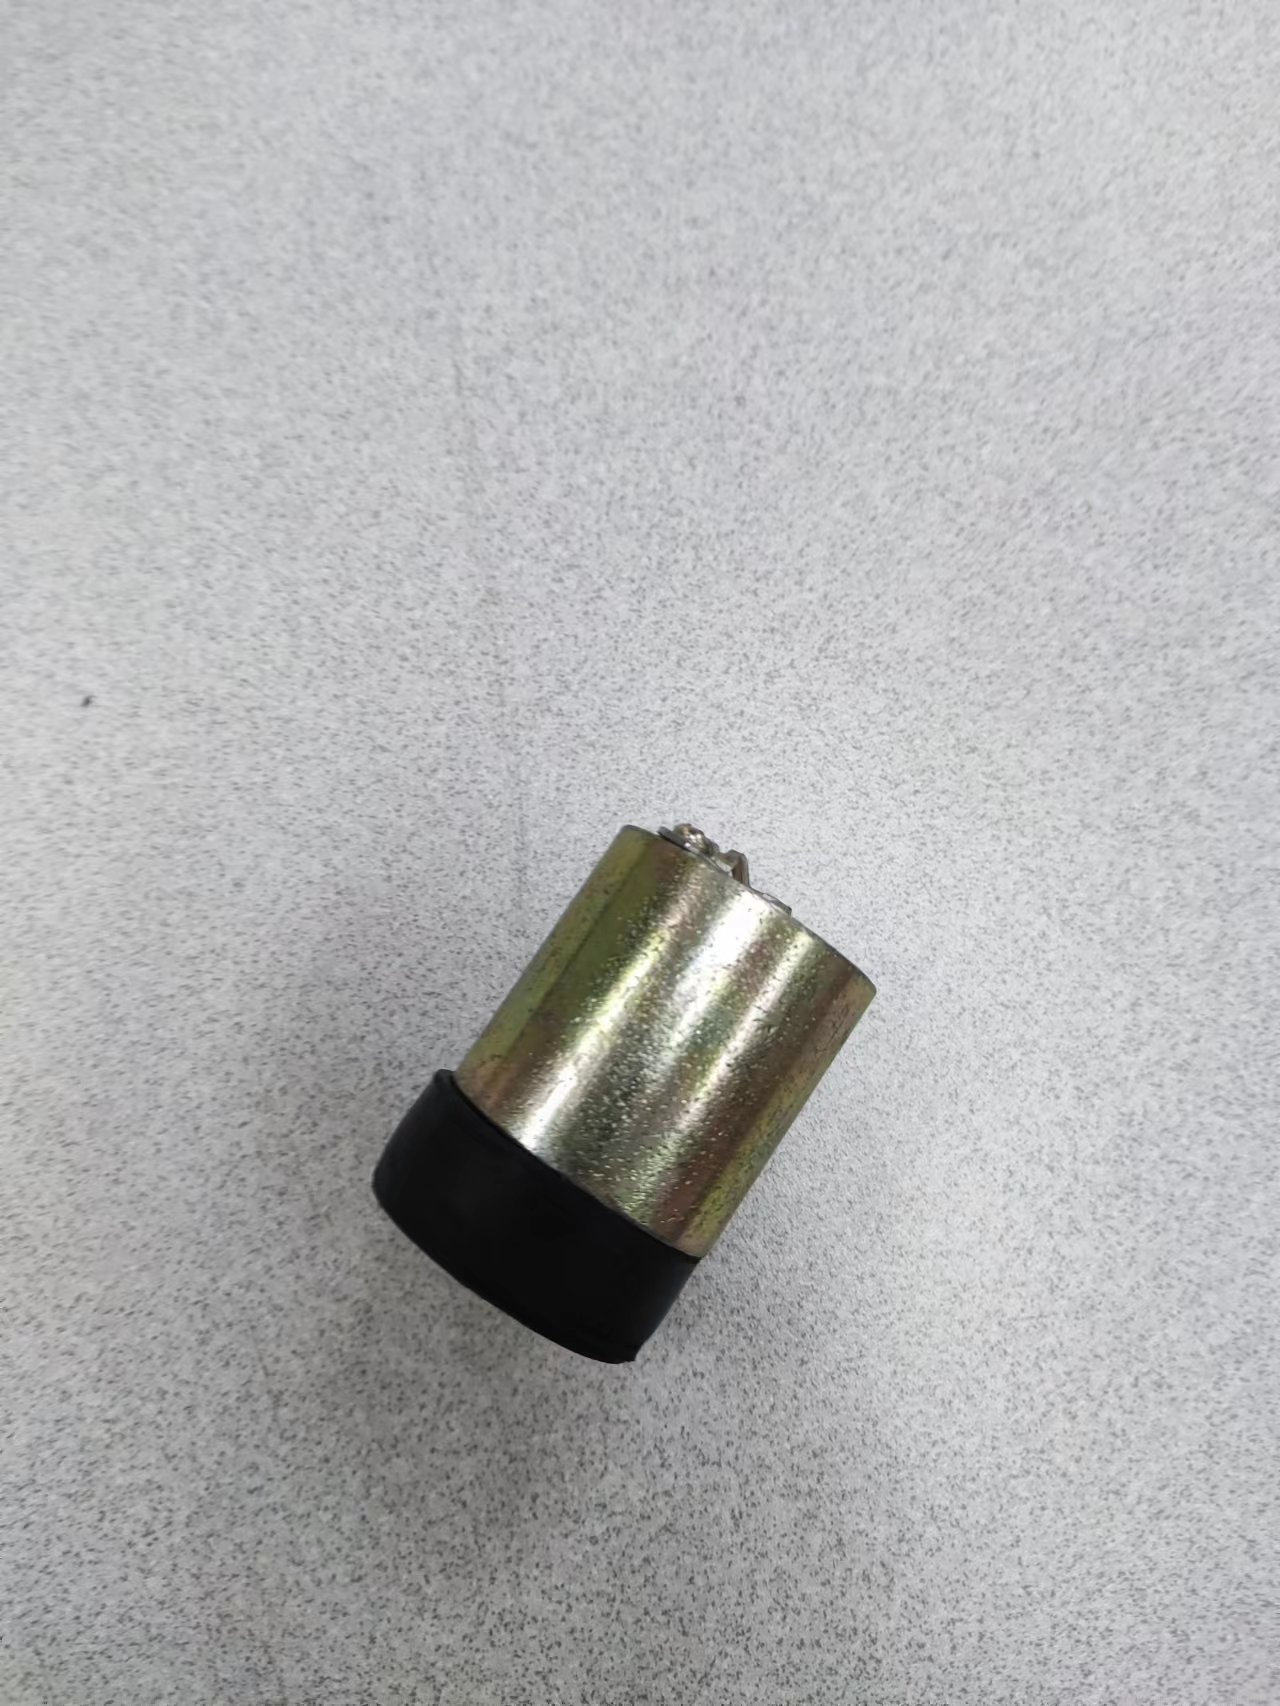
\includegraphics[width=0.30\textwidth]{2621669167980_.pic.jpg}}
    \subfigure[ticker-timer]{
    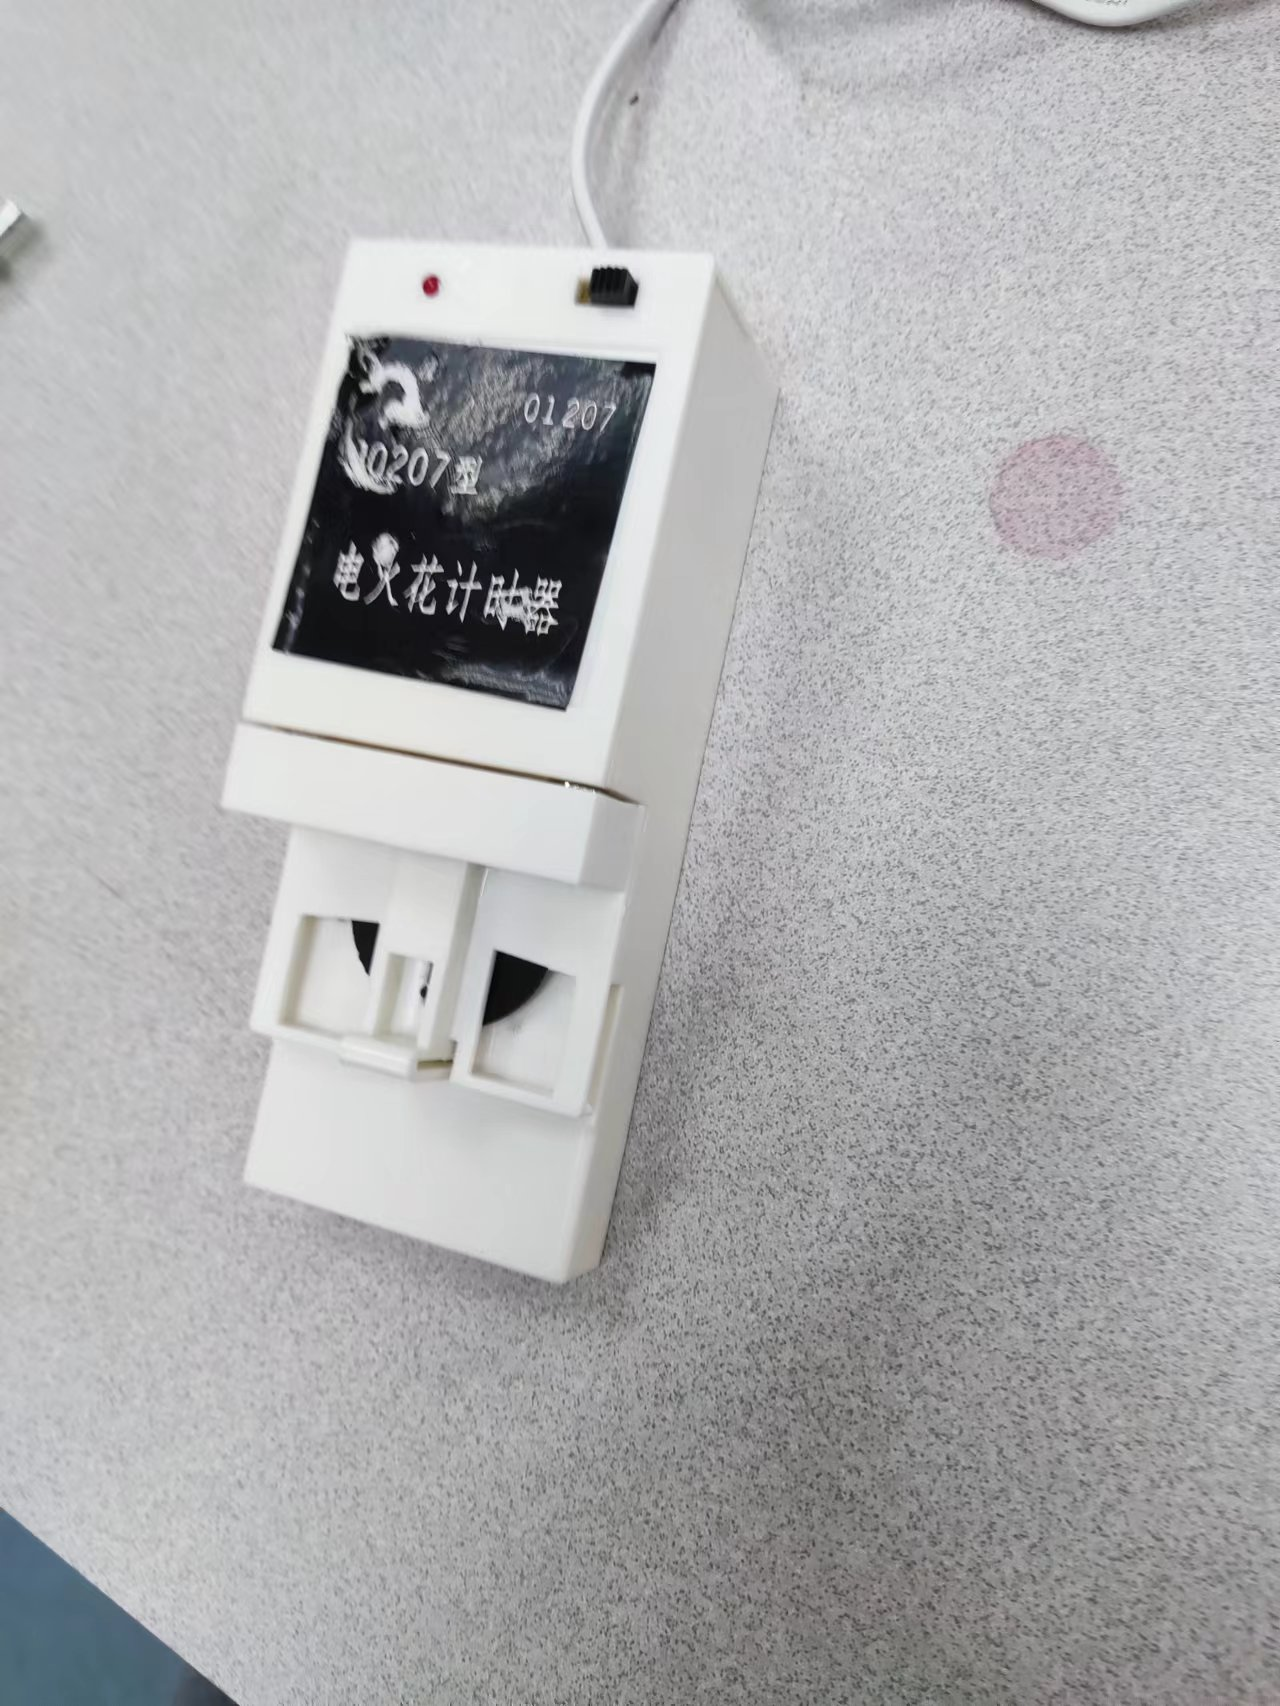
\includegraphics[width=0.30\textwidth]{2641669167981_.pic.jpg}}
    \caption{Instruments}
    \end{figure}
\section{Result of the Experiment}
\subsection{Collected Data}
\subsubsection{Procedure}
I pick eight dots from the tape, between the adjacent two there are three intervals,
meaning the time between the two is $0.06s$.\par
Then I measure the distance from the first to each of the rest ones and carry out the 
table below.
\subsubsection{Raw Data Table}
\begin{table}[!ht]
    \centering
    \begin{tabular}{|l|l|}
    \hline
        \textbf{Time$(s)$} & \textbf{Displacement$(\pm 0.5)(cm)$} \\ \hline
        0.06  & 1.4  \\ \hline
        0.12  & 5.9  \\ \hline
        0.18  & 13.8  \\ \hline
        0.24  & 24.9  \\ \hline
        0.3  & 39.3  \\ \hline
        0.36  & 57.2  \\ \hline
        0.42 & 78.4 \\ \hline
    \end{tabular}
    \caption{Raw Data Table}
\end{table}
\subsection{Processed Data }
\subsubsection{Average Instantaneous Velocity}
After obtaining the data from the experiment, we can determine their instantaneous velocity with uncertainty.\par
Given the equation that:
$$
v_i= \frac{\Delta d}{\Delta t}
$$\par
The time interval considered to be $0.06s$ , and the displacement between intervals can 
be calculate
by using the total displacement from this one to subract the one from the former 
interval.
\par
Thus we get the instantaneous velocity of the six period to be 
$23.3cms^{-1}, 75cms^{-1}, \\ 131.7cms^{-1}, 
185cms^{-1},  240cms^{-1},  298.3cms^{-1} and\ 353.3cms^{-1}$
, respectively.\par
\subsubsection{Uncertainty of $v_i$}
Similarly, since the way of determining percentage uncertainty is:\par
$$
Percentage  \ Uncertainty = \frac{\Delta u}{\overline{u}} \ \ \ \ 
\Delta v = \left| Percentage \ Uncertainty \right| \times \overline{v} 
$$\par
all the $\Delta v $ from the result are approxiamtely $8.3cms^{-1}$.\par 
\subsubsection{Processed Data Table}
\begin{table}[!ht]
    \centering
    \begin{tabular}{|l|l|l|}
    \hline
        \textbf{Time$(s)$ } & \textbf{Displacement$_i(\pm0.5)(cm)$ } &
         \textbf{Velocity$_i(\pm 8.3)(cms^{-1}$)} \\ \hline
        0.06  & 1.4  & 23.3  \\ \hline
        0.12  & 4.5  & 75  \\ \hline
        0.18  & 7.9  & 131.7  \\ \hline
        0.24  & 11.1  & 185  \\ \hline
        0.3  & 14.4  & 240  \\ \hline
        0.36  & 17.9  & 298.3  \\ \hline
        0.42 & 21.2 & 353.3 \\ \hline
    \end{tabular}
    \caption{Raw Data Table}
\end{table}
Note: the subsript i here means instantaneous.
\subsubsection{Acceleration due to Gravity}
The calculation of the acceleration is based on the \hyperlink{Graph1}{V-t Graph}.
Because the gradient of the tangent line of the V-t graph gives the instantaneous
acceleration.\par
From the graph the gradient of the best fit line is $922.5cms^{-2}$.
\hypertarget{my result}{\subsubsection{Uncertainty of Acceleration}}
Similar to above, the maximum and minmum gradient line has 
$964.7cms^{-2}$ and $874.6cms^{-2}$ as their slope. The maximum difference
between them and the best fit line's is $47.9cm^{-2}$. \par
Therefore, the acceleration with uncertainty is computed to be $922.5\pm 47.9cm^{-2}$.
\newpage
\section{Graphs}

\subsection{S-t Graph}


\begin{figure}[H]
    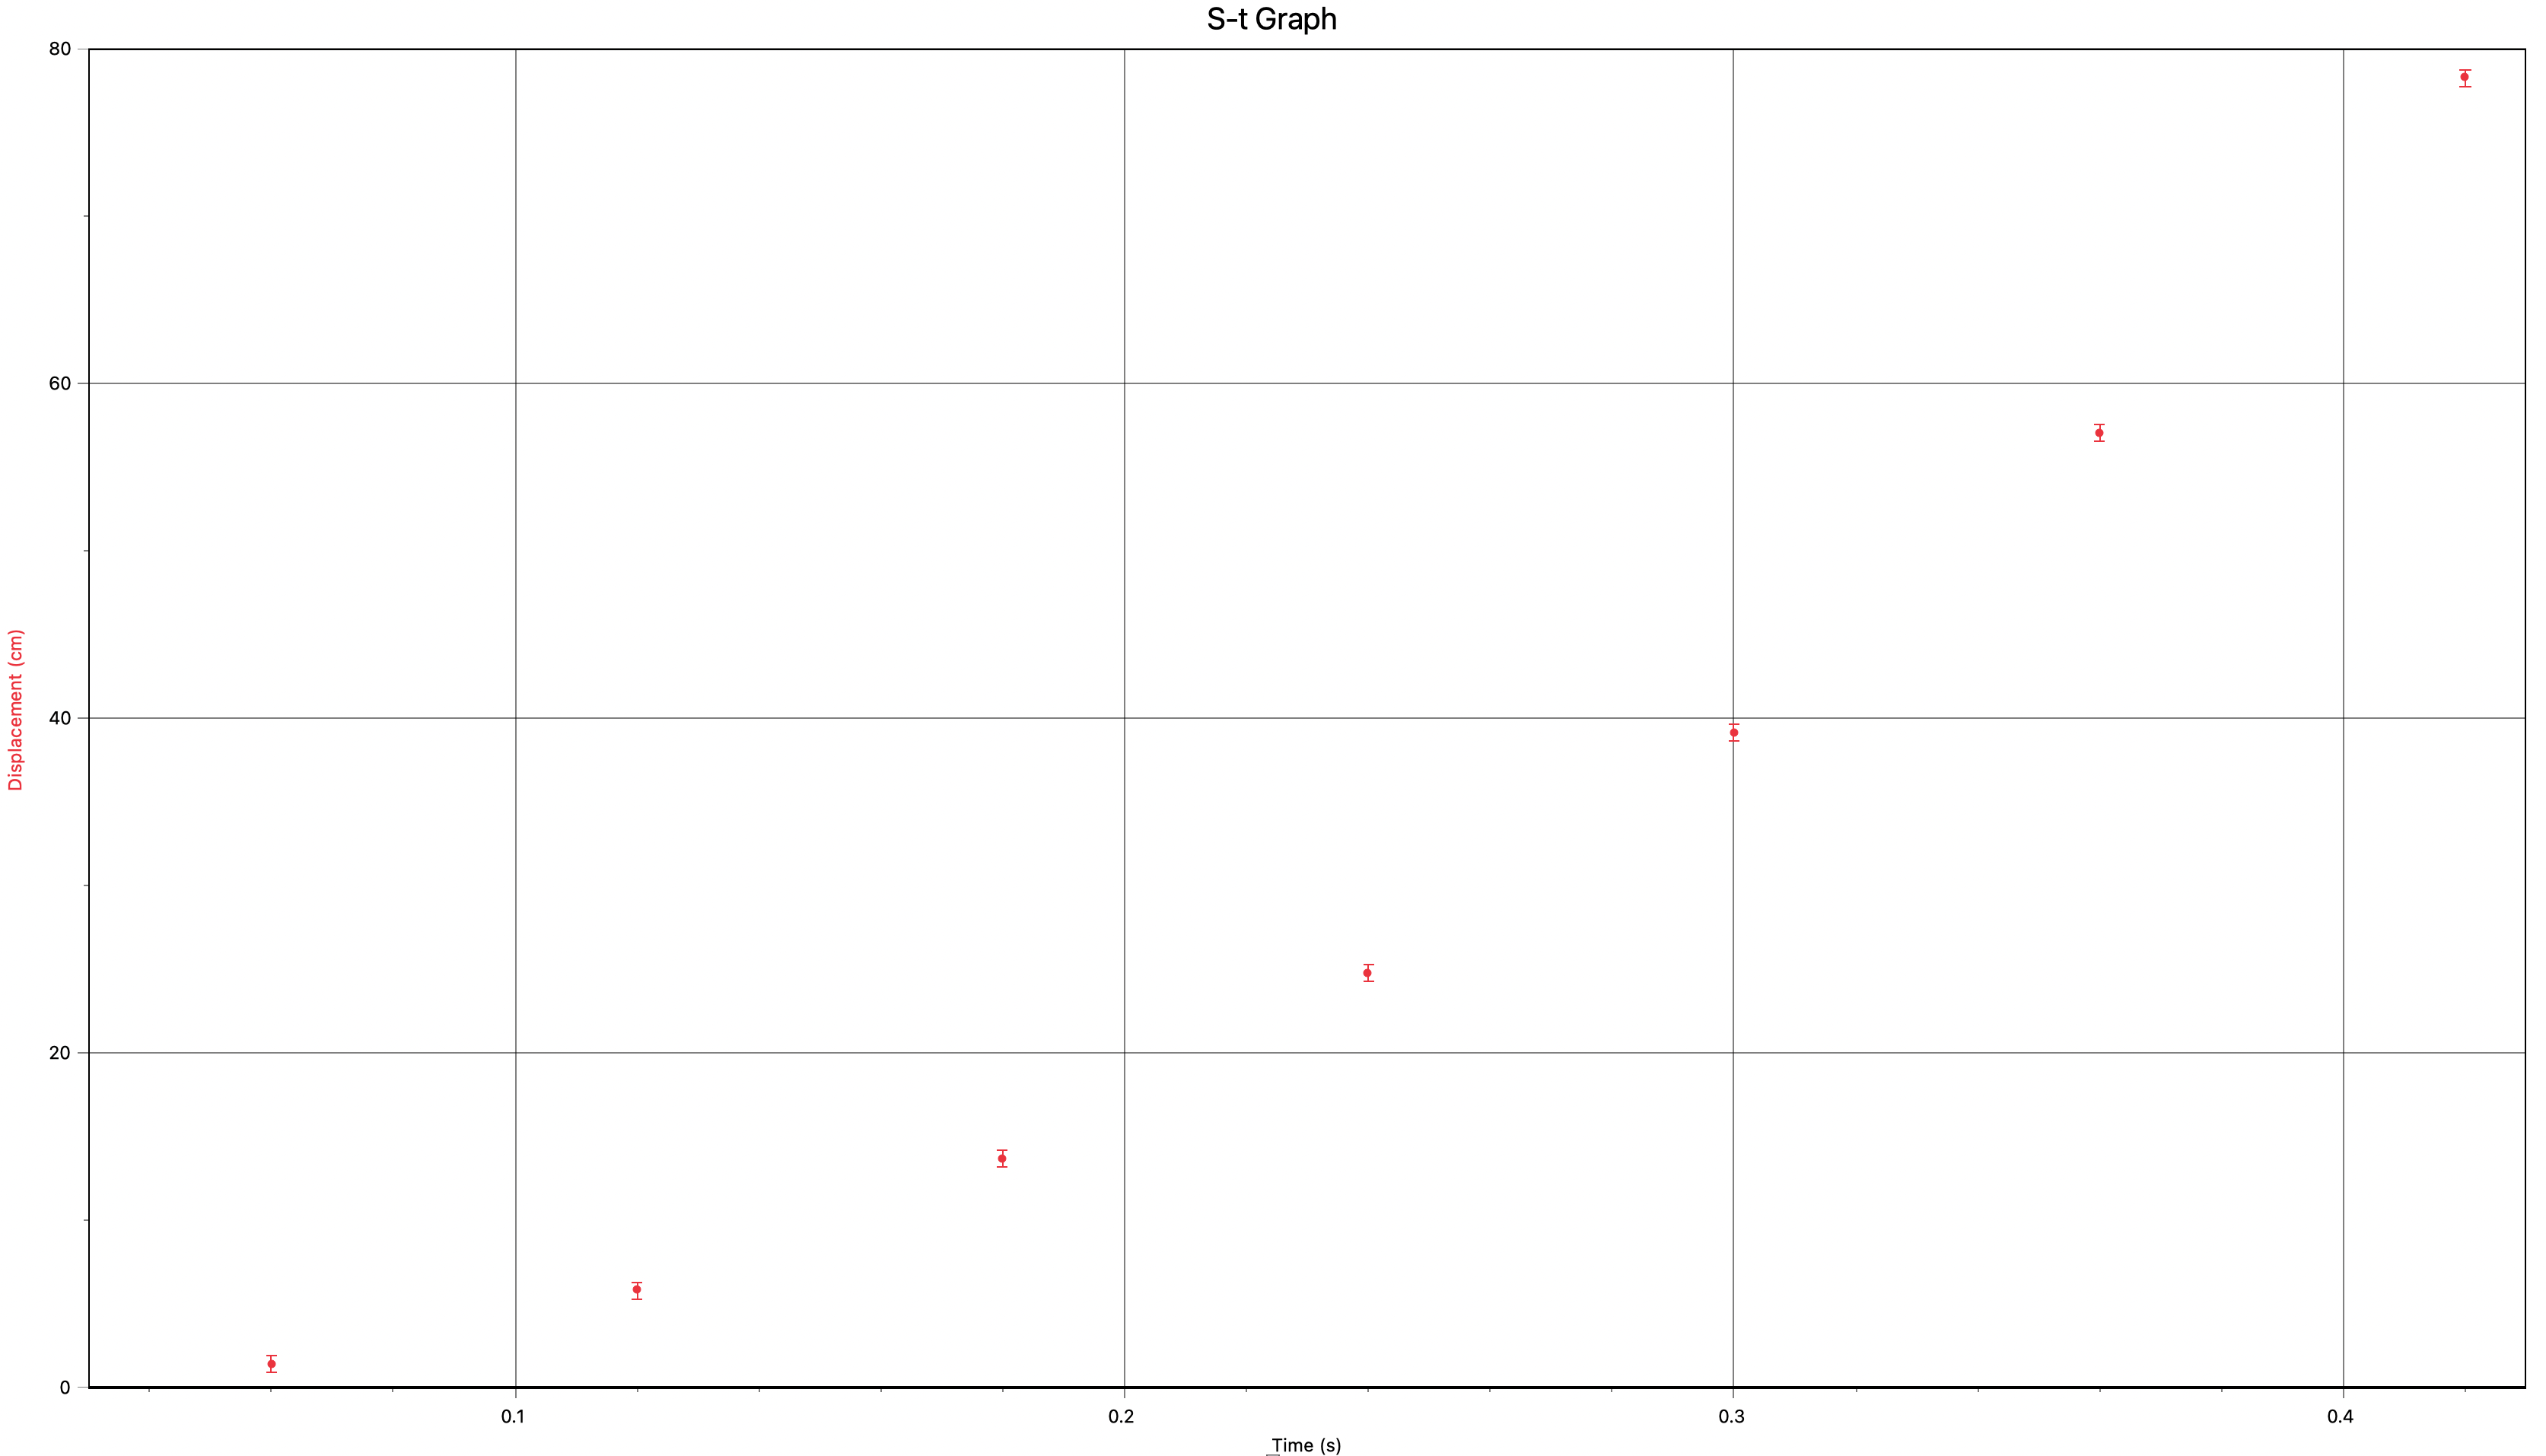
\includegraphics[width = 16cm, height = 12.5cm]{S-t.png}
    \caption{S-t Graph}
\end{figure}
\subsection{S-t$^2$ Graph}
\begin{figure}[H]
    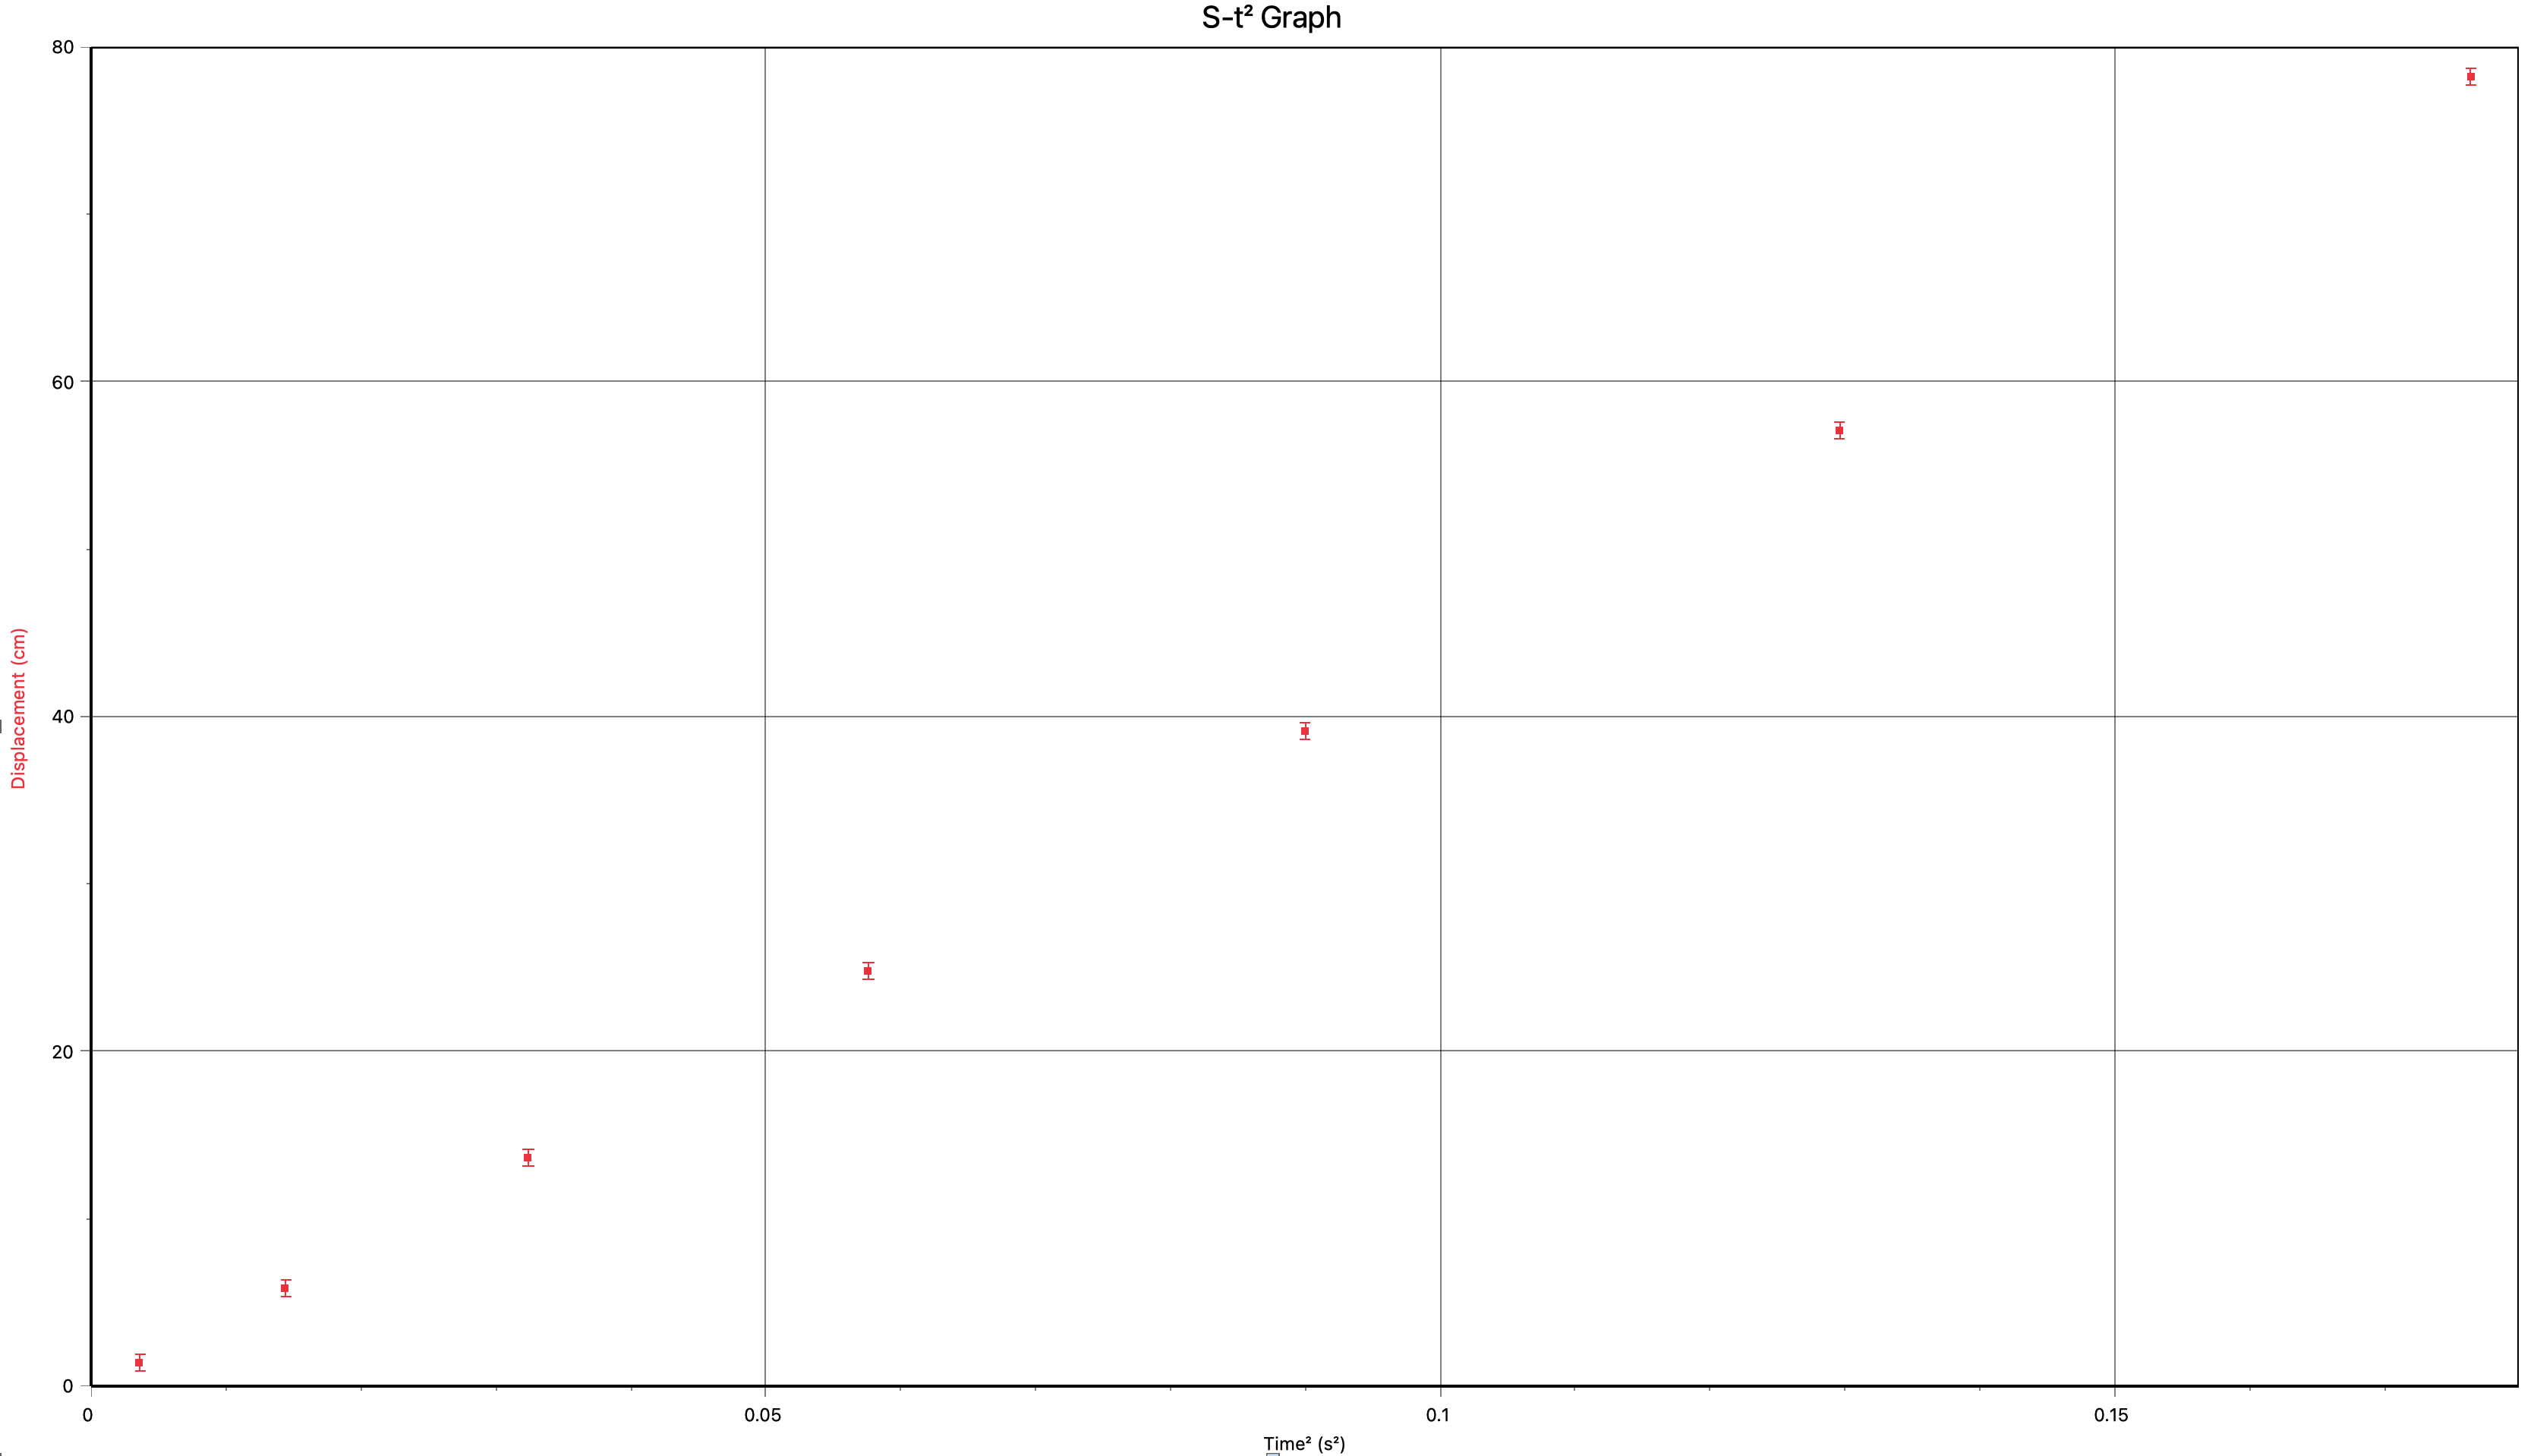
\includegraphics[width = 16cm, height = 12.5cm]{S-t^2.png}
    \caption{S-t$^2$ Graph}
\end{figure}
\hypertarget{Graph1}{\subsection{V-t Graph}}
\begin{figure}[H]
    \centering
    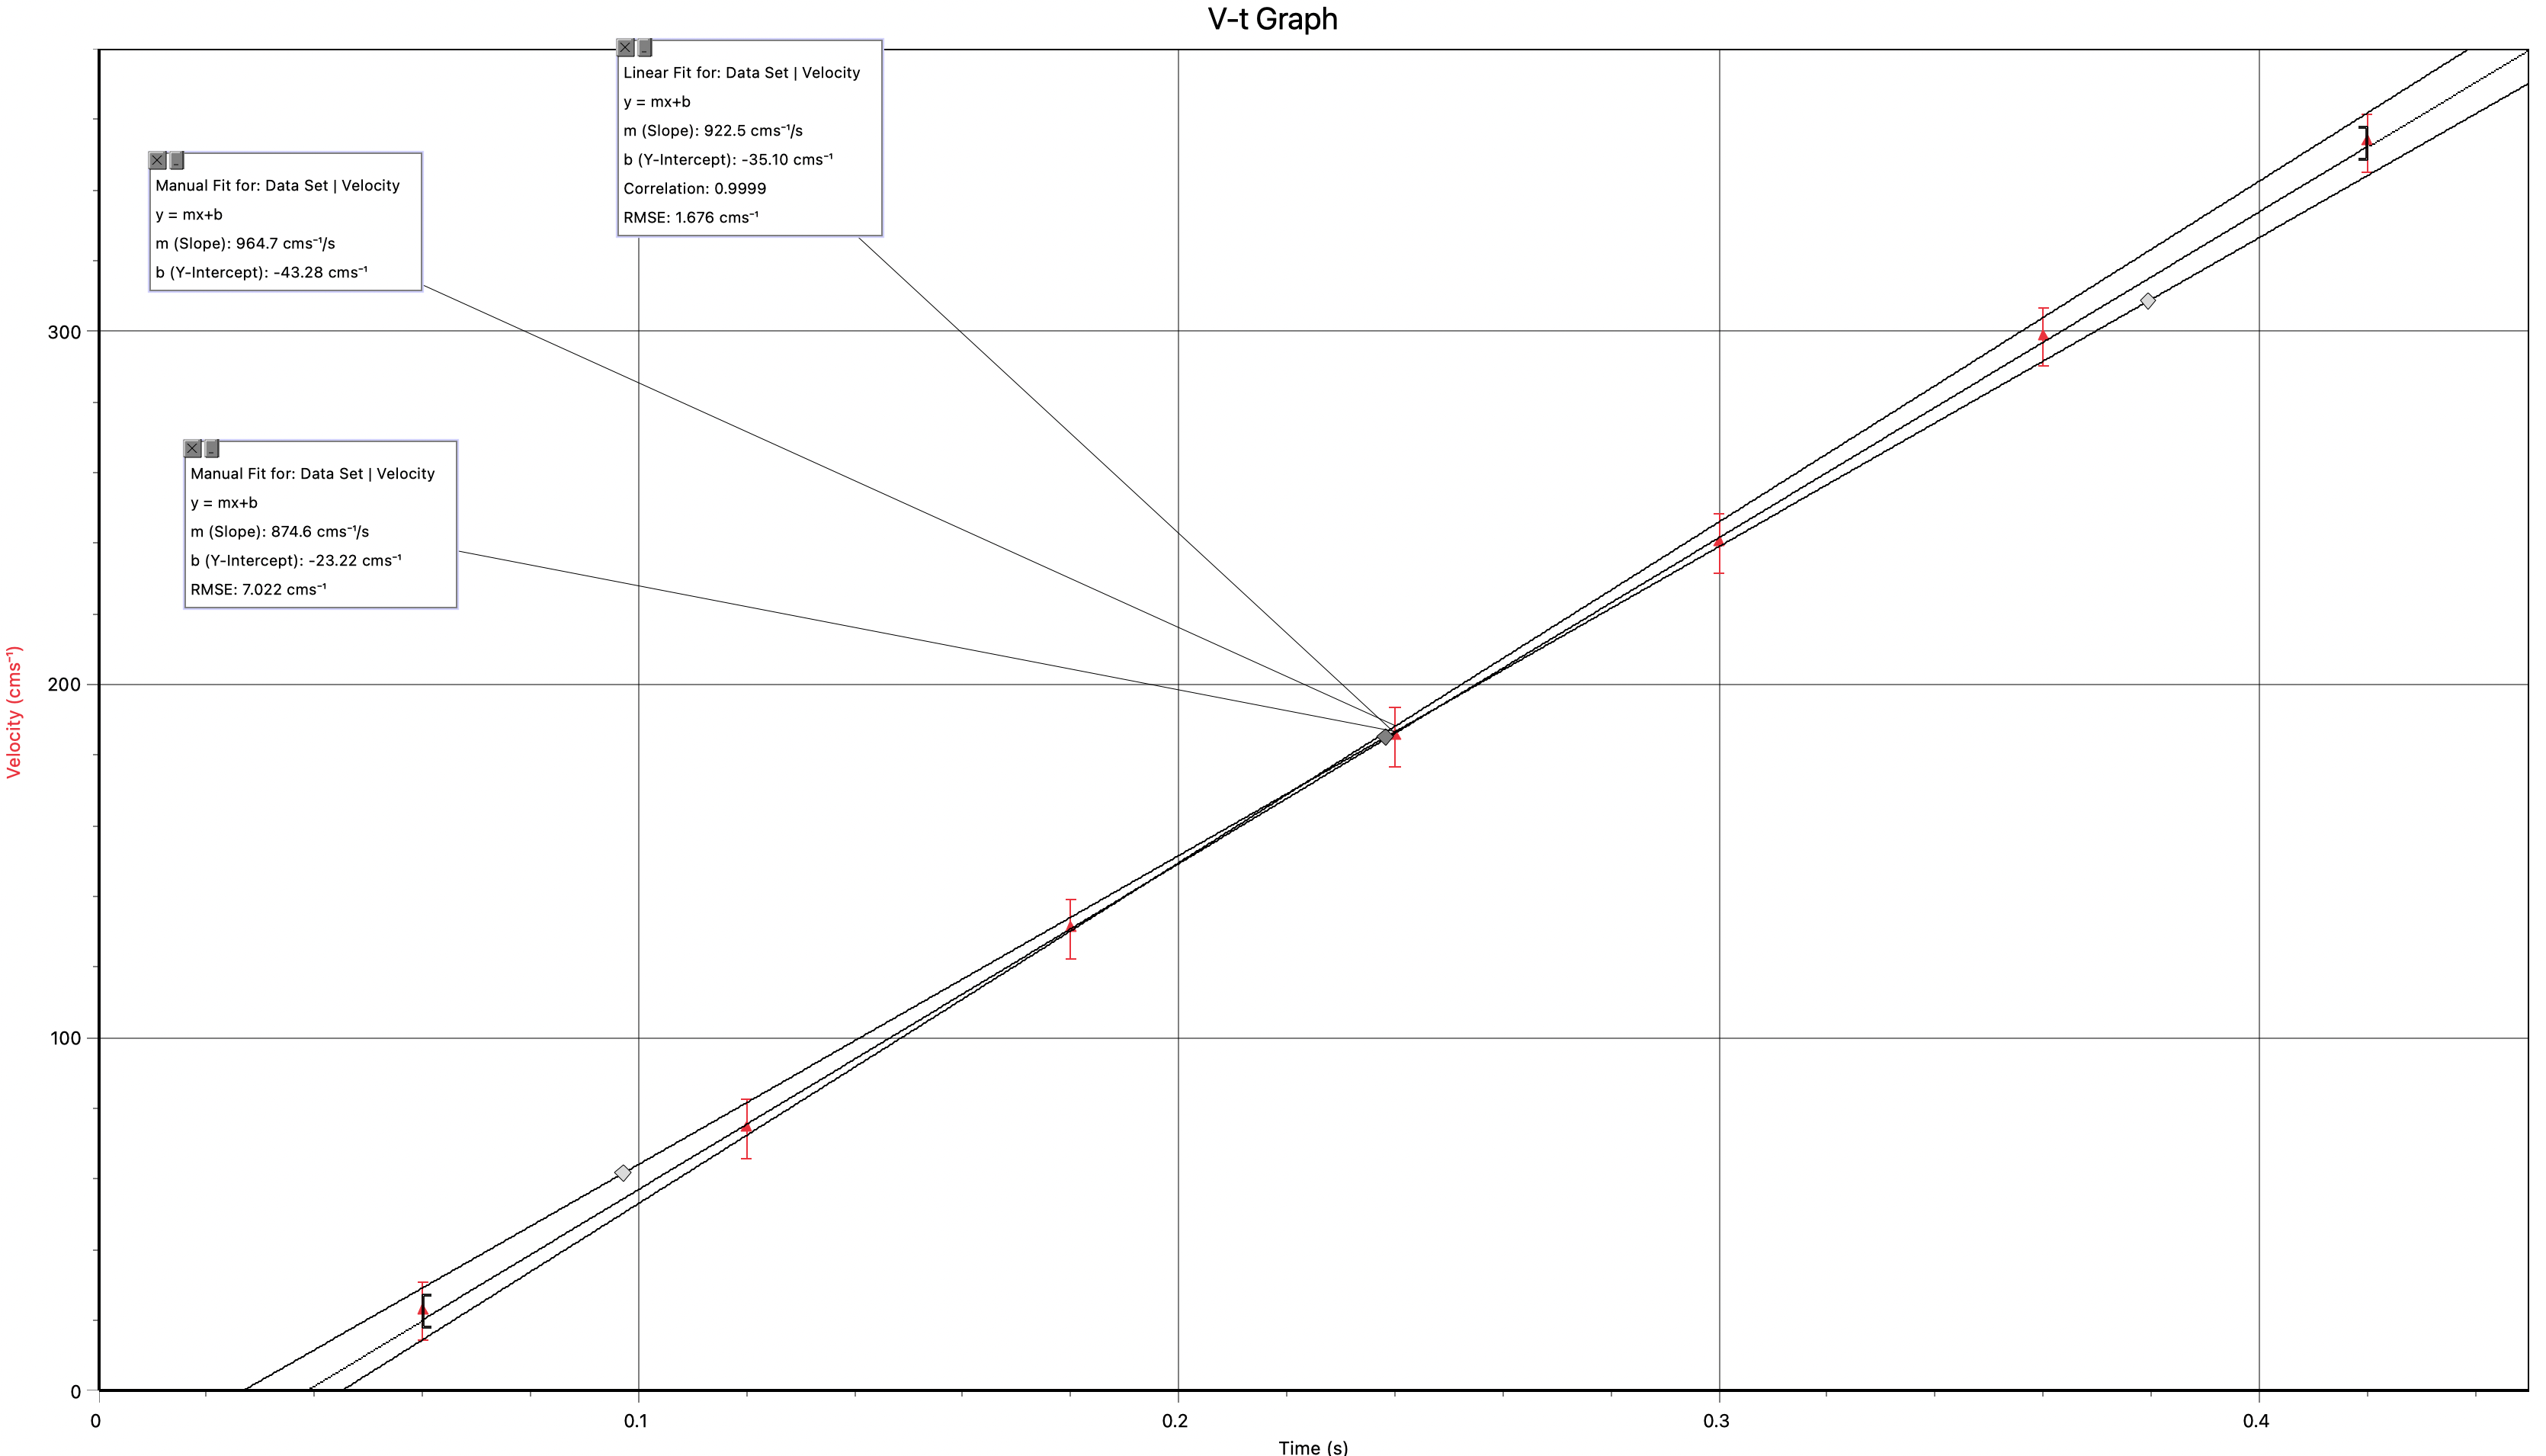
\includegraphics[width = 16cm, height = 12.5cm]{V-t Graph.png}
    \caption{V-t Graph}
\end{figure}
\section{Conclusion and Evaluation}
\subsection{Therotical Value}
After searching for some information online, I know that the gravitational acceleration 
should be close to around $981cm^{-2}$. And because gravitational acceleration on earth 
is constant, the instantaneous velocity of an falling object should be proportional to
the time spent falling.
\subsection{Experimental Result}
The data from \hyperlink{my result}{my result} however shows that g, the gravitational 
acceleration is $922.5\pm 47.9cms^{-2}$. The actual value is apparently out of this
range.
\subsection{Reflection}
After the whole investigation, I come up with several possible reasons that cause the 
difference between my result and the therotical one.\par
A possible one is maybe due to the limit of tools. The meter I use is not
precise enough for the measuring the distances between dots, leading to the
inaccurate conclusion.\par
Perhaps another one is on account of the ievitable random error. I only measured once
throughtout the experiment. So there is possiblitiy that the raw data I get is not that
precise.\par
I will try my best to avoid the problems above in the next investigation so as to
work out a more precise conclusion.
\end{document}

